
\section{Problemstellung}

IT ist aus dem Alltag schon seit den 1980er Jahren nicht mehr wegzudenken. Wie oben bereits angedeutet, hat der Gewinn an Produktivität und Bequemlichkeit, den die Welt durch den Einsatz von IT erreicht hat, einen Preis: Jeder Computer und jedes Datenpaket, das über das Internet versendet wird, benötigt Strom. Zunächst soll erläutert werden, inwiefern hier ein Problem entstanden ist, das sich in Zukunft deutlich verschärfen wird, und wie daraus die Ziele der vorliegenden Arbeit abgeleitet werden.

\subsection{Motivation}
Obwohl der Stromverbrauch der OECD-Staaten seit mehreren Jahren stagniert oder sogar leicht zurück geht, steigen die globalen Verbräuche weiter an (vgl. Abbildung \ref{fig:ProbStromSektor}). Das kann vor allem auf  Schwellenländer zurückgeführt werden, die in kurzer Zeit ein rasantes wirtschaftliches Wachstum erleben.

\begin{figure}[htb]
	\centering
	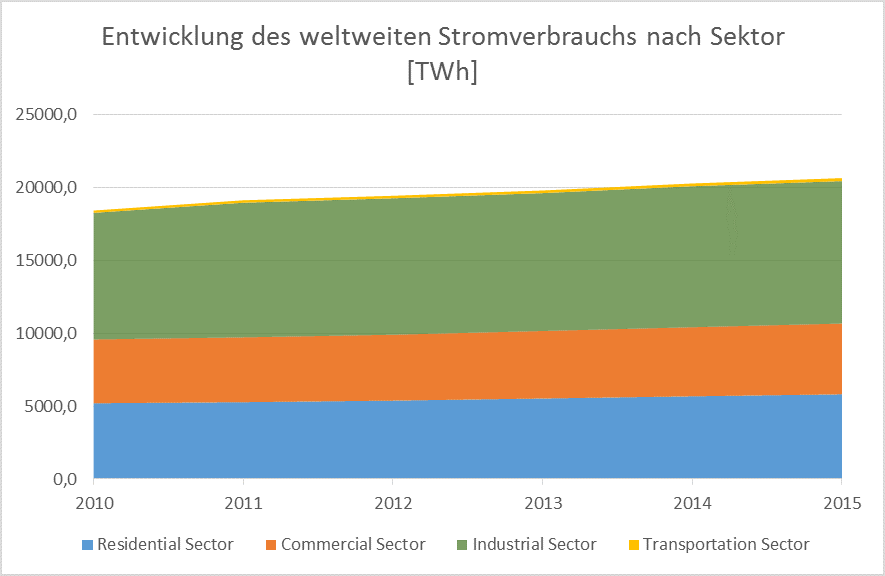
\includegraphics[width=0.8\textwidth]{ProbStromSektor}
	\caption{Weltweiter Stromverbrauch nach Sektoren, nach \cite{eia2016}}
	\label{fig:ProbStromSektor}
\end{figure}
Da aller Bemühungen zum Trotz die fossilen, nicht regenerierbaren Energieträger Erdöl, Kohle und Erdgas weiterhin ca. 81 Prozent der weltweiten Energieerzeugung ausmachen \cite{statista}, sind langfristig steigende Energiekosten \cite[40\psqq]{iea2015} ein großes Risiko für ICT-Provider weltweit, die insgesamt mit steigenden Kosten zu kämpfen haben.

Steigende Energiekosten für sich genommen wären schon ein starkes Argument, Netze effizienter zu gestalten.  Der Effekt der Kosten wird allerdings potenziert durch den Fakt, dass der Stromverbrauch von ICT von 2007 bis 2012 stärker gewachsen ist als der globale Stromverbrauch \cite[9]{vanhedde}. Schon 2012 betrug der Anteil von ICT am globalen Stromverbrauch etwa 5\% (s. Abbildung \ref{fig:ProbStromICT})

\begin{figure}[htb]
	\centering
	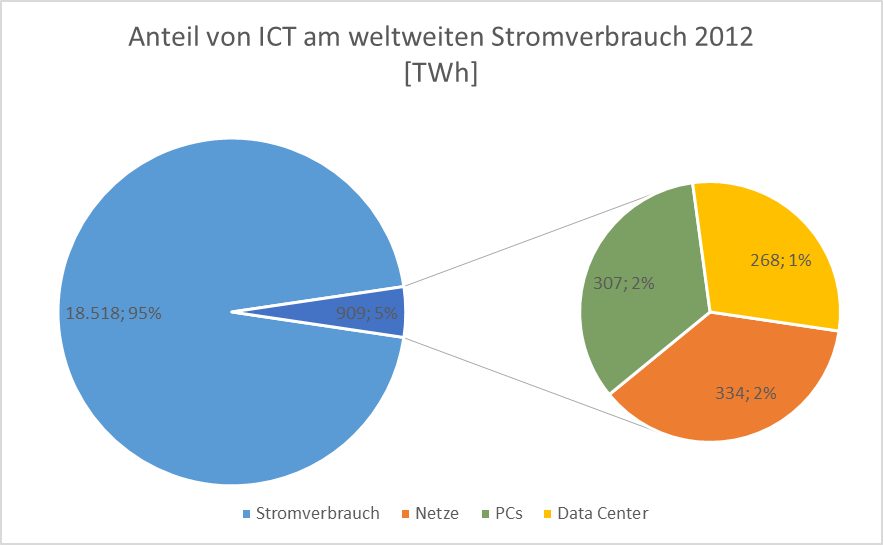
\includegraphics[width=0.8\textwidth]{ProbStromICT}
	\caption{Anteil von ICT am weltweiten Stromverbrauch, basierend auf \cite{eia2016} und \cite{vanhsheet}}
	\label{fig:ProbStromICT}
\end{figure}

Seit dem ist der Anteil der Weltbevölkerung, der das Internet verwendet, von 20,6\% (2007) auf 43,4\% (2015) gestiegen \cite{itu}. Ein Wachstum, das sich in der näheren Zukunft nicht verlangsamen wird. Weiterhin sorgen steigende Datenvolumen pro Nutzer für eine immer größer werdende Netzlast. Welchen Effekt die Industrie 4.0 und das Internet der Dinge (englisch: Internet of Things, kurz: IoT) auf die Netze weltweit haben werden, lässt sich momentan  noch nicht abschätzen. Eins jedoch steht fest: Das Netz der Zukunft wird mehr Daten zu bewältigen haben als jemals zuvor.

Die genannten Entwicklungen bedrohen die Geschäftsmodelle von Telekommunikationsanbietern und Netzbetreibern. Angesichts sinkender Preise und steigender Kosten ist es notwendig, die  Kosteneinsparungspotenziale energieeffizienter Netzkonzepte und -technologien zu ermitteln. So kann die Infrastruktur, auf die mittlerweile so große Teile der Wirtschaft beruhen, weiterhin profitabel betrieben werden.

\subsection{Ziele}
Das Ziel der vorliegenden Arbeit ist es, abzuschätzen, wie viel Energie  durch Verwendung energieeffizienter Technologien eingespart werden kann und welche Kostensenkungen sich daraus erzielen lassen.

Dazu ist zu Beginn eine Literaturrecherche zu den bestehenden Technologien nötig, die es ermöglichen, den Energieverbrauch von Netzen zu senken.

Anschließend soll eine Software entwickelt werden, die es ermöglicht, zwei hypothetische Netze miteinander zu vergleichen. Als Ausgangspunkt dient dabei ein konventionelles Netz, wie es heutzutage Stand der Technik ist. Damit verglichen wird ein energieeffizientes Netz, das die vorhandenen Technologien und Konzepte zur Effizienzsteigerung sinnvoll einsetzt. Anhand des abgeschätzten Energieverbrauchs der beiden Netze wird das Energiesparpotenzial sowie die möglichen Kosteneinsparungen durch den Betrieb des energieeffizienten Netzes ausgegeben. 

Die Softwarelösung wird als objektorientierte Java Desktop Anwendung mit einer Einteilung der Klassen in die drei Bereiche Model, View und Controller implementiert.

Der Prozess der Softwareentwicklung soll nach dem Wasserfallmodell ablaufen. Die Programmaufteilung und geforderten Funktionen sind bereits vor der Implementierung hinreichend bekannt, so dass die Anwendung eines agilen Entwicklungsmodells hier keine entscheidenden Vorteile bietet. 

Zunächst werden in den folgenden Kapiteln aktuelle Konzepte und Technologien vorgestellt, mit denen die Energieeffizienz von Netzen erhöht werden kann.
